\section{Transfer Back to Driving}
\label{sec:transfer}

Can the measured error structure improve driving gaze beyond the
median offset, and can acquisition qualify what it records (RQ3, C3)?

\begin{figure*}[t]
\centering
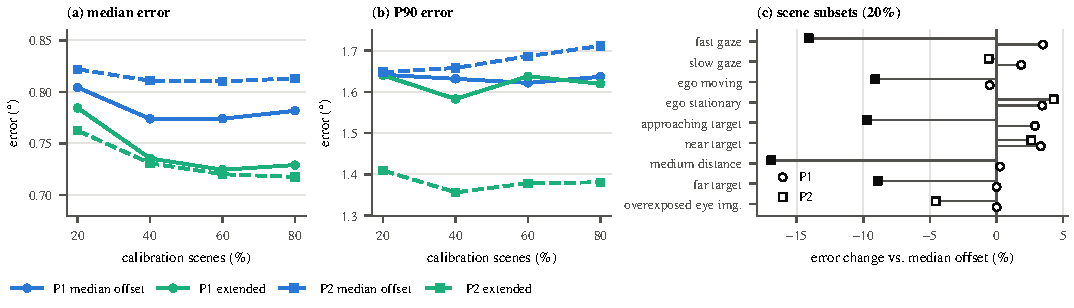
\includegraphics[width=\textwidth]
    {figures/fig4_transfer.pdf}
\caption{Per-wearer correction versus the median-offset baseline on
held-out driving scenes. (a) Median and (b) P90 error as the calibration
share grows, averaged over repeated random splits. (c) Change in error
per scene subset at 20\% calibration; filled markers are significant
after Benjamini--Hochberg correction.}
\label{fig:transfer}
\end{figure*}

\textbf{Corrections matched to the error structure.}
The controlled study suggests two mechanisms: a position-dependent bias
term for the spatial effects and causal temporal filtering for
pursuit-like dispersion. The median offset is a strong baseline, so we
select one candidate per participant on calibration scenes only. At 20\%
calibration, the median error falls from 0.80\dg{} to 0.78\dg{} for P1
(2.5\%, better in 14 of 16 splits) and from 0.82\dg{} to 0.76\dg{} for
P2 (7.3\%, 16 of 16; Fig.~\ref{fig:transfer}a). With 40--80\%
calibration scenes, the gains grow to 5--7\% and 10--12\%. The
participants benefit from different mechanisms: P1 increasingly from the
spatial bias term, P2 from a causal 50\,ms trailing median filter. This
supports selecting corrections per wearer rather than assuming one
mechanism for everyone.

\textbf{Largest gains in dynamic scenes.}
For P2, the correction also trims the tail: P90 falls by 14\% at 20\%
calibration (1.65\dg{} to 1.41\dg{}) and by 18--19\% with more
references (Fig.~\ref{fig:transfer}b). The gains concentrate in fast gaze
movements, approaching targets and a moving ego vehicle
(Fig.~\ref{fig:transfer}c), consistent with the pursuit dispersion
measured in the controlled study. For P1, gains are smaller and come from
the spatial term. Simple corrections matched to the measured errors thus
add value without a new gaze estimator.

\textbf{Quality-aware acquisition.}
Correction alone does not tell whether a sample suits a downstream task.
The acquisition pipeline therefore annotates each sample with
transparent suitability flags. A segmentation model separates windshield,
side windows and mirrors from the vehicle interior; scene sharpness
(Laplacian variance), optical flow and IMU motion characterise image
degradation; and eye openness, blinks and gaze dynamics mark periods in
which the eye may be poorly visible. The original measurements are kept,
so each task selects what it needs. In an initial test on four recordings
of one participant (28\,min), viewing-region, eye-openness and sharpness
gates retained 82\% of the time in intervals of at least 0.5\,s. This
shows the coverage the gates leave; their effect on angular accuracy
remains to be measured.

\textbf{Lightweight in-situ accuracy checks.}
Because a few verified fixations already estimate the offset well
(Sec.~\ref{sec:realworld}), the same automatically generated references
can check accuracy during acquisition, for example after the glasses are
put on again, and indicate when the correction should be updated. This
is a practical check, not a guarantee of continuous accuracy.
